Jēdzientelpas no teksta korpusa iegūst ar neironu tīkliem, kuri uztver kontekstu no tuvākajiem vārdiem tekstā.

Continuous Bag-of-Words (CBOW) un Continuous Skip-gram Model ir divas neironu tīklu modeļu arhitektūras jēdzientelpu izveidei balstoties uz teksta korpusa. Metožu priekšrocība ir tajā, ka nav nepieciešama anotēta treniņu datu kopa, trenēšanai izmanto lielus teksta korpusus. CBOW modelī apkārt esošos vārdus izmanto vidū esošā vārda paredzēšanai. Skip-gram modelī vārda vektoru izmanto konteksta paredzēšanai (\ref{fig:cbow-skipgram} attēls).

\begin{figure}[h]
	\centering
	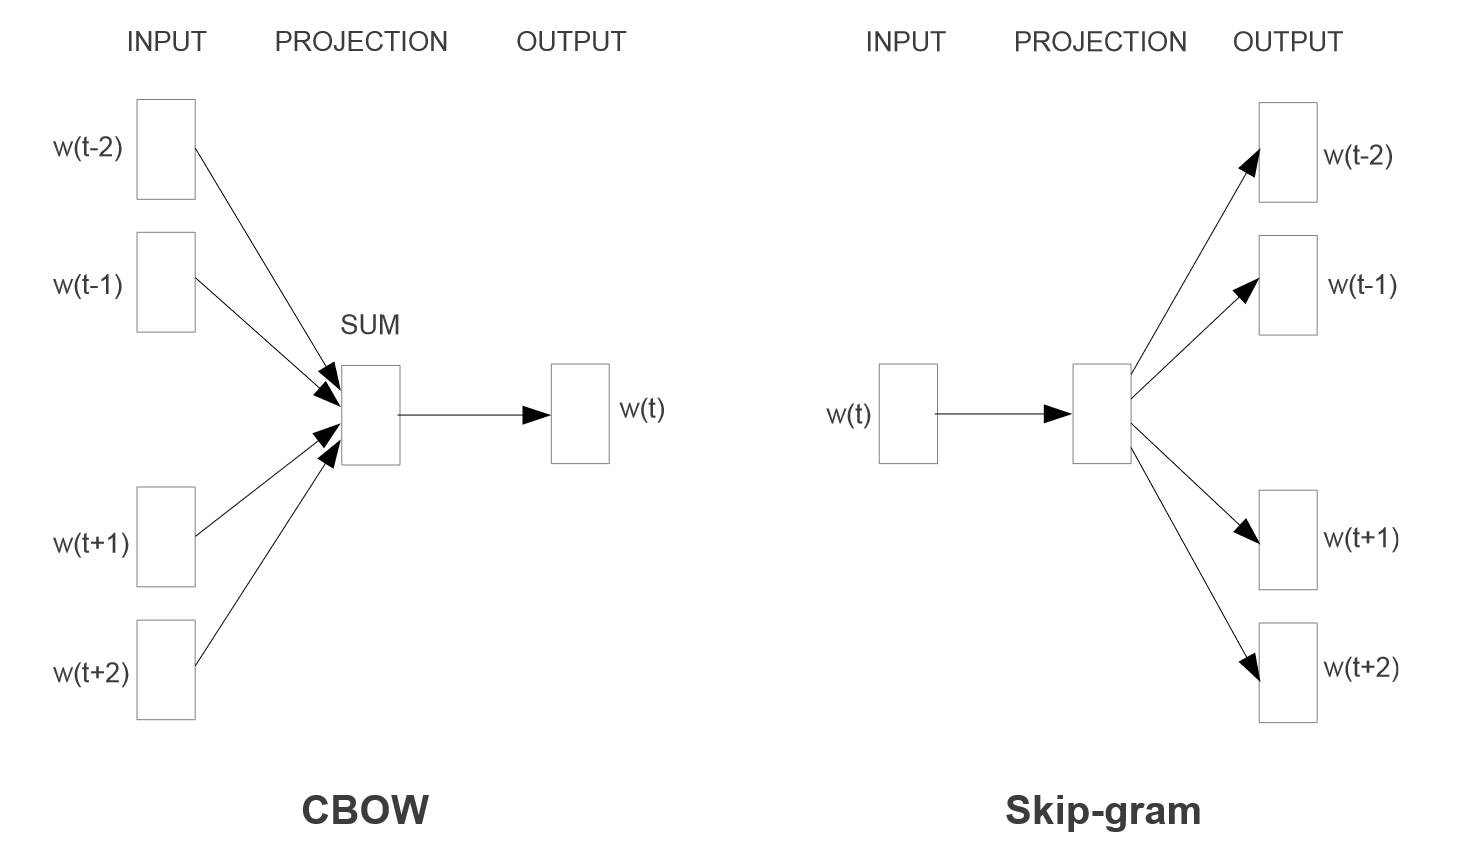
\includegraphics[width=\textwidth]{figures/word2vec-models.png}
	\caption{CBOW un Skip-gram modeļu arhitektūra \cite{word2vec2013}.}
	\label{fig:cbow-skipgram}
\end{figure}




% Ideja un cosine of the angle
% \url{https://en.wikipedia.org/wiki/Vector_space_model}

% test \cite{mikolov2013exploiting}.


\section{Continuous Bag-of-Words}

Bag-of-Words (BOW) apzīmē vārdu grupu nesaglabājot kārību. Vienā izlasē (bag) vārda tuvums mērķa vārdam konkrētā izlasē nav tik svarīgs, atkārtojot procesu uz korpusa no konteksta tāpat tiks sīkāk (granulētāk) izšķirti svari tuvākajiem vārdiem, piemēram, Rīga un Latvija būs tuvumā 1000 reizes biežāk nekā Rīga un sniegs.
% \url{https://en.wikipedia.org/wiki/Bag-of-words_model}

CBOW (Continuous Bag-of-Words) metodē neironu tīkls mēģina uzminēt esošo (vidējo) vārdu no $n$ iepriekšējiem un $n$ nākošajiem vārdiem. Procesu atkārtojot, vārdiem, kas bieži parādās vienā kontekstā, būs līdzīgi vektori. Pēc izkliedētības (\textit{distributional}) hipotēzes vārdi, kas atrodas līdzīgos kontekstos, ir ar līdzīgu nozīmi \cite{word2vec2013}. Tāpat kā BOW modelī, CBOW vārdu secība neietekmē projekciju. Nepārtrauktība (\textit{continuuity}) modelī rodas no tā, ka izmanto nepārtrauktu izkliedētu konteksta reprezentāciju
% (continuous distributed representation of the context)
jeb svari starp ievades un projekcijas slāņiem tiek lietoti visiem vārdiem.
% (weight matrix between the input and the projection layer is shared for all word positions) 
\cite{word2vec2013}.

\section{Continuous Skip-gram Model}


Koncepts ir uztrenēt neironu tīklu ar slēpto slāni (\textit{hidden layer}) un iegūt slēptā slāņa svarus, kas patiesībā arī ir vārdu vektori. Uzdevums ir no ievades vārdu pa vārdam paredzēt apkārt esošos vārdus. Kaimiņu vārdu skaits -- loga izmērs (\textit{window size}) -- ir hiperparametrs (\ref{fig:skipgram} attēls).

% [piemērs]

\begin{figure}[h]
	\centering
	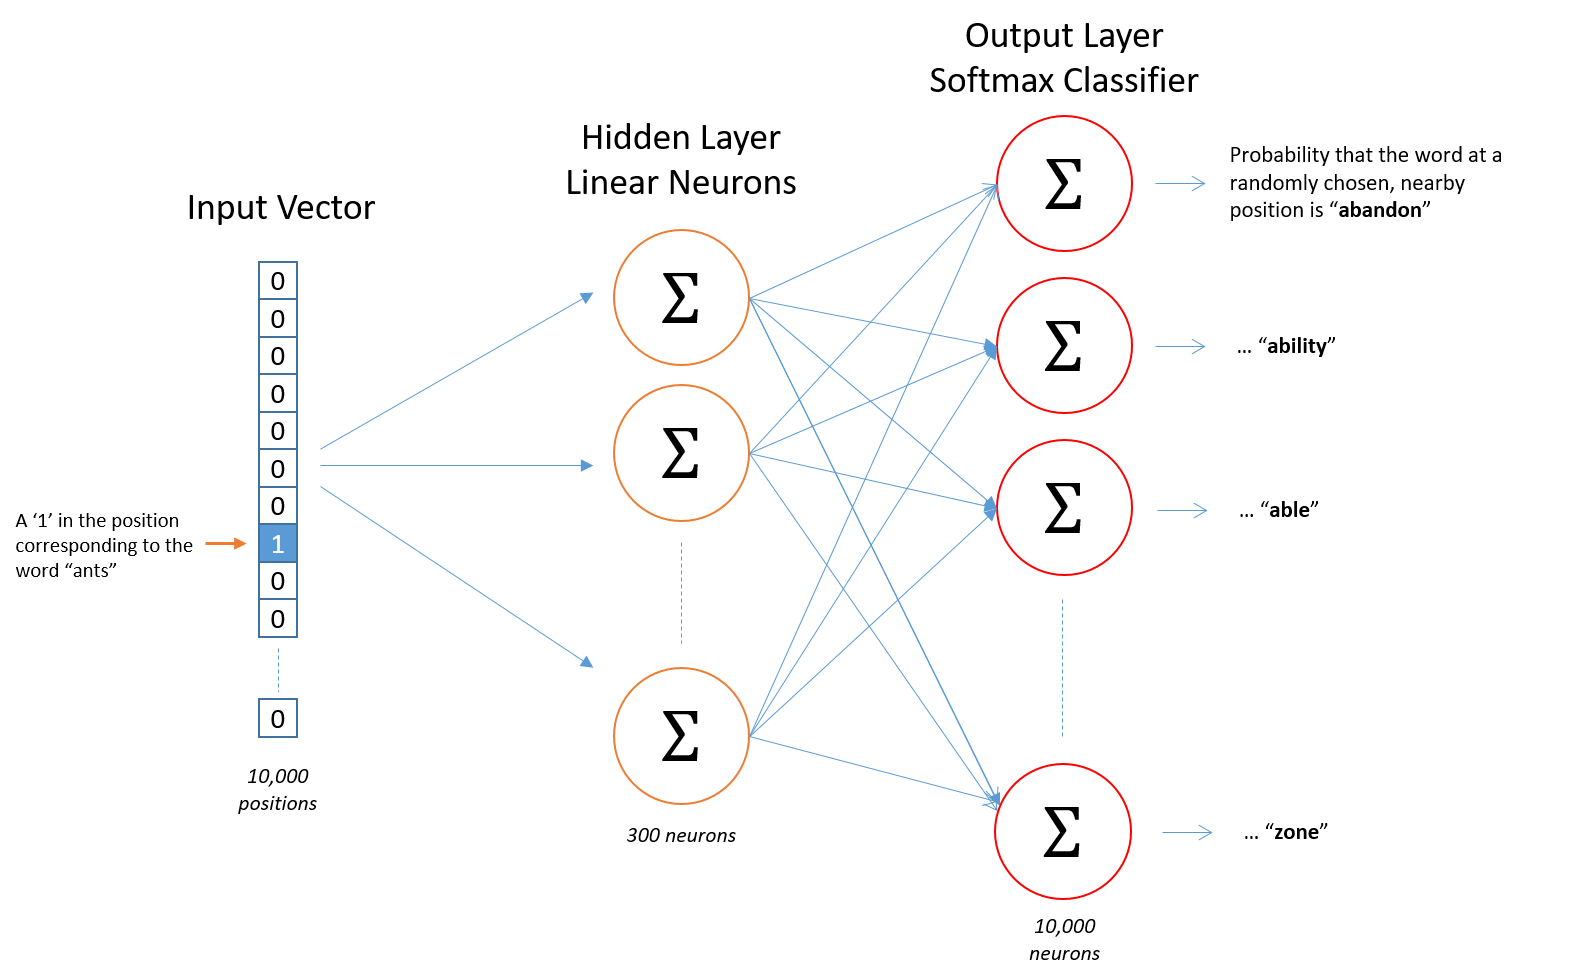
\includegraphics[width=\textwidth]{figures/skip_gram_net_arch.png}
	\caption{Skip-gram modeļa arhitektūra.
	Ievades vektors -- vārda vienizcēluma kodējums $1xn$ -- kur $n$ ir vārdu skaits; 
	slēptais slānis --  $nxl$, kur $l$ ir loga izmērs;
	Softmax slānis -- $1xl$;
	Izvades slānis -- $1xn$ \cite{mccormick2016}.}
	\label{fig:skipgram}
\end{figure}

% \section{Modeļu performance/salīdzinājums/rezultāti}

% Metožu priekšrocība ir tajā, ka nav nepieciešama anotēta treniņu datu kopa, trenēšanai izmanto lielus teksta korpusus.


% "Skip-gram works well with a small amount of the training data, represents well even rare words or phrases.
% CBOW several times faster to train than the skip-gram, slightly better accuracy for the frequent words." 
% \url{https://groups.google.com/g/word2vec-toolkit/c/NLvYXU99cAM/m/E5ld8LcDxlAJ}
